\documentclass[a4paper,11pt]{article}
\usepackage{graphicx,tikz}
\usepackage[most]{tcolorbox} 
\usepackage{multirow}
\usepackage{enumitem}
\usepackage{amssymb}
\usepackage{amsmath}
\usepackage{setspace}  
\usepackage{varwidth}
\usepackage{amsthm}
\usepackage{xcolor}
\usepackage{multicol}
\usepackage{multirow}
\usepackage{array}
\usepackage{animate}
\usepackage{amsthm}
\usepackage{caption}
\usepackage{minted}
\usepackage{forest}
\usepackage{fancyhdr}
\usepackage{geometry}
\geometry{
		total = {160mm, 237mm},
		left = 15mm,
		right = 10mm,
		top = 10mm,
    bottom = 15mm,
    headheight=2cm
	}

\renewcommand{\headrulewidth}{0pt}
\newcommand{\R}{\mathbb{R}}
\newcommand{\N}{\mathbb{N}}
\newcommand{\Z}{\mathbb{Z}}
\newcommand{\Q}{\mathbb{Q}}
\newcommand{\jawab}{\textbf{Solusi}:}

\usetikzlibrary{graphs, shapes, arrows.meta, positioning}


\definecolor{bg}{rgb}{0.95, 0.95, 0.92}
\definecolor{pastelblue}{RGB}{173,216,230}
\definecolor{pastelpink}{RGB}{255,182,193}
\definecolor{pastelmint}{RGB}{152,251,152}

\setminted[cpp]{bgcolor=bg,frame=single,bgcolorpadding=1mm,escapeinside=||}

\title{Try out OSK Informatika}
\author{17 Mei 2025}
\date{}

\begin{document}
\maketitle
\begin{enumerate}
  \item \textbf{Mengambil Daun}
  
  Pak Dengklek dan Pak Ganesh bergiliran memainkan permainan ``mengambil daun''. Daun-daun ditumpuk pada dua piring: A dan B. Pada piring A terdapat 2 lembar daun dan pada piring B terdapat 3 lembar daun.

\begin{center}
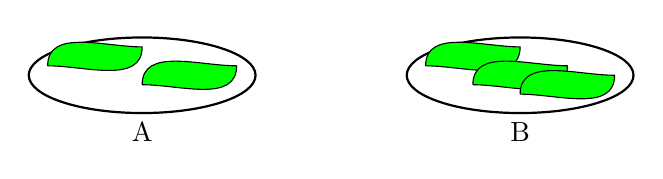
\begin{tikzpicture}[scale=1.2]
  % Piring A
  \draw[thick] (-2,0) ellipse (1.2 and 0.4);
  \node at (-2, -0.6) {A};

  % Piring B
  \draw[thick] (2,0) ellipse (1.2 and 0.4);
  \node at (2, -0.6) {B};


  % Daun di piring A
  \draw[fill=green]  (-3,0.1)  to [out=90,in=180] (-2,0.3) to [out=270,in=0](-3,0.1);
  \draw[fill=green]  (-2,-0.1)  to [out=90,in=180] (-1,0.1) to [out=270,in=0](-2,-0.1);

  % Daun di piring B
  \draw[fill=green]  (1,0.1)  to [out=90,in=180] (2,0.3) to [out=270,in=0](1,0.1);
  \draw[fill=green]  (1.5,-0.1)  to [out=90,in=180] (2.5,0.1) to [out=270,in=0](1.5,-0.1);
  \draw[fill=green]  (2,-0.2)  to [out=90,in=180] (3,0) to [out=270,in=0](2,-0.2);
\end{tikzpicture}
\end{center}

\vspace{0.5em}

Saat gilirannya, pemain harus mengambil 1 atau lebih daun dari salah satu piring. Pemenang permainan ini adalah pemain yang mengambil daun terakhir dari 5 lembar daun yang ada.

\vspace{1em}

Dari 5 skenario kondisi awal permainan berikut, manakah yang menjamin kemenangan Pak Dengklek?

\begin{enumerate}[label=\Alph*.]
  \item Pak Dengklek memulai permainan dengan mengambil 1 daun dari piring A
  \item Pak Dengklek memulai permainan dengan mengambil 2 daun dari piring A
  \item Pak Dengklek memulai permainan dengan mengambil 2 daun dari piring B
  \item Pak Ganesh memulai permainan dengan mengambil 1 daun dari piring A
  \item Pak Ganesh memulai permainan dengan mengambil 1 daun dari piring B
\end{enumerate}

  \item \textbf{Menulis Alfabet}
  \begin{center}
    \begin{tcolorbox}[enhanced, width=0.55\textwidth]
\ttfamily\noindent\centering\large
ABCDEFGHIJKLMNOPQRSTUVWXYZAAABACADAEAFAG
AHAIAJAKALAMANAOAPAQARASATAUAVAWAXAYAZBA
BBBCBDBEBFBGBHBIBJBKBLBMBNBOBPBQBRBSBTBU
BVBWBXBYBZCACBCCCDCECFCGCHCICJCKCLCMCNCO
CPCQCRCSCTCUCVCWCXCYCZDADBDCDDEDFDGDHDID
JDKDLDMDNDODPDQDRDSDTDUDVDWDXDYEZAEBCEDE
EEFEGEHEIEJEKELEMENEOEPEQERESETEUEVWEXEY
EZFABFBCFDEFEFFFGFHFIFJFKFLFMFNFOPPFQFRF
SFTFUFVFWFXFYFZGAGBGCGDGEGFGGGHGHGIGJ\ldots
\end{tcolorbox}
  \end{center}


Pak Blangkon memiliki spidol papan tulis yang sedari dulu tintanya tidak pernah habis. Karena Pak Blangkon 
berniat ingin membeli spidol lagi, ia berencana untuk menghabiskan tinta spidolnya itu. Strateginya adalah ia 
akan terus menulis alfabet di papan tulis dengan spidolnya sampai tintanya habis. Pak Blangkon menuliskan 
alfabet dengan cara sebagai berikut:

\begin{itemize}
    \item Pertama, Pak Blangkon menuliskan semua permutasi dari 1 buah alfabet (A, B, \ldots, Z).
    \item Kemudian, ia menuliskan semua permutasi dari 2 buah alfabet (AA, AB, \ldots, AZ, BA, \ldots, ZZ).
    \item Kemudian, ia menuliskan semua permutasi dari 3 buah alfabet (AAA, \ldots, ZZZ).
    \item Proses tersebut dilakukan hingga tinta spidolnya habis.
\end{itemize}

Ternyata setelah strateginya dilakukan, tinta spidolnya habis pada huruf ke-2025. Huruf apakah itu?

\textbf{Jawaban:} \underline{\hspace{2cm}} \quad \emph{(tuliskan jawaban dalam bentuk HURUF ALFABET saja)}

\item \textbf{Persebaran Virus}

Diberikan sebuah diagram yang merepresentasikan sebuah jaringan komputer sebagai berikut:
\begin{center}
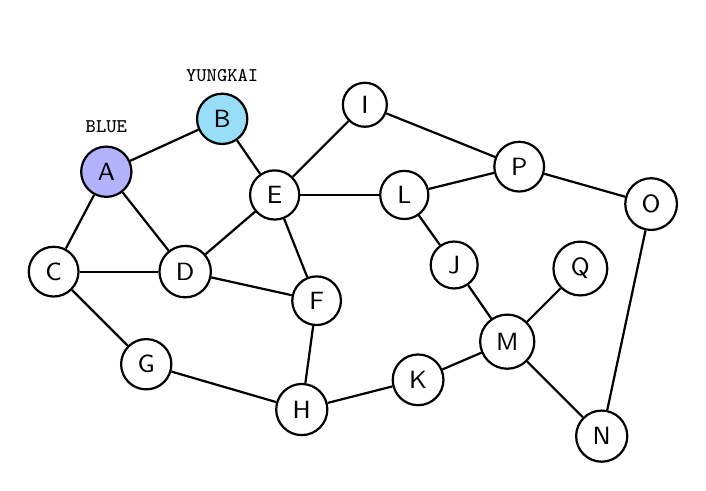
\begin{tikzpicture}[>=Stealth, node distance=1cm, every node/.style={circle, draw, minimum size=0.5cm}, thick,font=\small\sffamily]

% Nodes
\node[fill=blue!30] (A) {A};
\node[fill=cyan!40] [above right=0.2cm and 1cm of A] (B) {B};
\node [below left=0.8cm and 0.2cm of A] (C) {C};
\node [right=of C] (D) {D};
\node [below right=0.5cm and 0.2cmof B] (E) {E};
\node [below right=-0.1cm and 1.2cm of D] (F) {F};
\node [below right=of C] (G) {G};
\node [below right= 0.1cm and 1.5cm of G] (H) {H};
\node [above right=of E] (I) {I};
\node [above right=-0.1cm and 1cm of H] (K) {K};
\node [above right=1cm and 0cm of K] (J) {J};
\node [right=of E] (L) {L};
\node [below right= 0.5cm and 0.2cm of J] (M) {M};
\node [below right=of M] (N) {N};
\node [above right=-0.1cm and 1cm of L] (P) {P};
\node [above right= 0.6 cm of M] (Q) {Q};
\node [below right=0cm and 1.2cm of P] (O) {O};

% Edges
\draw (A) -- (B);
\draw (A) -- (C);
\draw (A) -- (D);
\draw (B) -- (E);
\draw (C) -- (D);
\draw (C) -- (G);
\draw (D) -- (F);
\draw (E) -- (F);
\draw (E) -- (L);
\draw (F) -- (H);
\draw (G) -- (H);
\draw (H) -- (K);
\draw (L) -- (P);
\draw (L) -- (J);
\draw (M) -- (Q);
\draw (M) -- (K);
\draw (M) -- (J);
\draw (M) -- (N);
\draw (P) -- (I);
\draw (I) -- (E);
\draw (O) -- (N);
\draw (O) -- (P);
\draw (D) -- (E);


% Labels
\node[above=-2mm of A,draw=none] {\scriptsize\texttt{BLUE}};
\node[above=-4mm of B,draw=none] {\scriptsize\texttt{YUNGKAI}};

\end{tikzpicture}
\end{center}

Komputer \textbf{A} terinfeksi dengan virus \texttt{`BLUE'} dan komputer \textbf{B} terinfeksi dengan virus \texttt{`YUNGKAI'}.

Pada pukul $00:00$ tiap harinya, masing-masing virus menyebar ke sembarang komputer (dapat bernilai lebih dari 1) yang terhubung langsung dengan komputer yang terinfeksi. Jika kedua virus bertemu pada sebuah komputer, maka komputer tersebut akan rusak dan tidak akan ada virus yang menyebar dari komputer yang rusak tersebut. Setelah beberapa hari, semua komputer akan terinfeksi atau rusak.

\medskip

Berapa banyak komputer yang terinfeksi oleh virus \texttt{`YUNGKAI'} setelah 7 hari?

\textbf{Jawaban:} \underline{\hspace{2cm}} \quad \emph{(tuliskan jawaban dalam bentuk ANGKA saja)}

\item \textbf{Perjalanan Drone}

Sebuah drone melakukan perjalanan yang dimulai dari sebuah kotak putih. Ia menghadap ke salah satu arah dari 4 kemungkinan arah yang ada.

\begin{center}
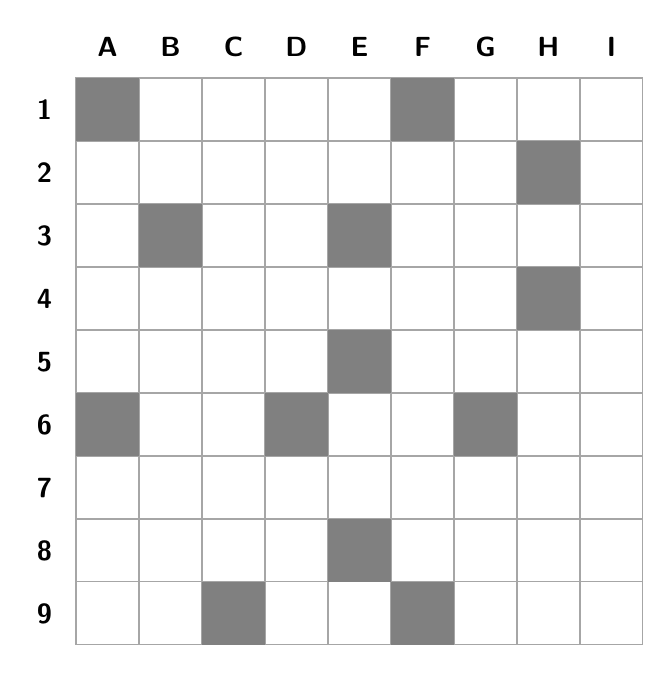
\begin{tikzpicture}[scale=0.8, font=\sffamily]
  \foreach \x in {1,...,9} {
    \foreach \y in {1,...,9} {
      \draw[gray!70] (\y,10-\x) rectangle ++(1,-1);
    }
  }

  % Kotak abu-abu
  \foreach \x/\y in {1/1, 2/3, 6/1, 8/2, 5/3, 8/4, 5/5, 1/6, 4/6, 7/6, 5/8, 3/9, 6/9} {
    \fill[gray] (\x,10-\y) rectangle ++(1,-1);
  }

  % Label kolom (A-I)
  \foreach \i [count=\j from 1] in {A,B,C,D,E,F,G,H,I} {
    \node at (\j + 0.5, 9.5) {\textbf{\i}};
  }

  % Label baris (1-9)
  \foreach \i in {1,...,9} {
    \node at (0.5,10-\i - 0.5) {\textbf{\i}};
  }
\end{tikzpicture}
\end{center}

Kemudian ia mengunjungi 9 kotak putih lainnya tanpa mengunjungi kotak abu-abu sama sekali dengan prosedur sebagai berikut:

\begin{enumerate}
  \item Maju tiga kotak ke depan.
  \item Hadap kiri 90 derajat (tetap di kotaknya saat ini).
  \item Maju empat kotak ke depan.
  \item Hadap kanan 90 derajat (tetap di kotaknya saat ini).
  \item Maju dua kotak ke depan.
\end{enumerate}

Berapakah banyaknya kemungkinan kotak awal/\textit{starting point} drone tersebut?

\textbf{Jawaban:} \underline{\hspace{2cm}} \quad \emph{(tuliskan jawaban dalam bentuk ANGKA saja)}

\item \textbf{Bermain Mesin Capit}

\begin{center}
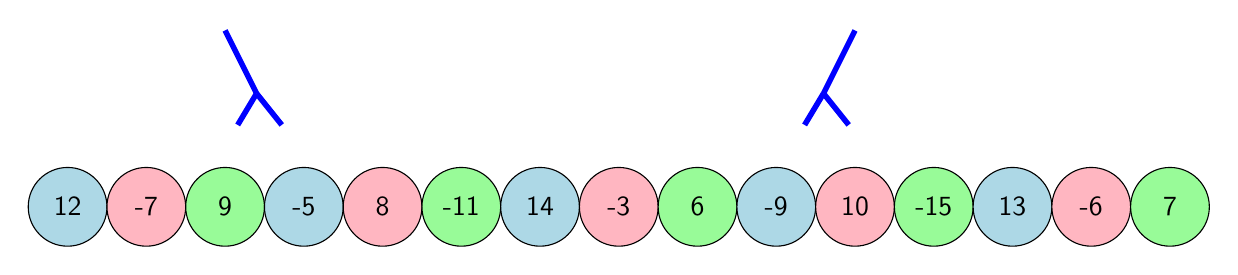
\begin{tikzpicture}[font=\sffamily,scale=0.8]
  % Gambar lengan capit sederhana
  \draw[line width=2pt, blue] (2.5,2) -- (3,1);
  \draw[line width=2pt, blue] (3,1) -- (3.4,0.5);
  \draw[line width=2pt, blue] (3,1) -- (2.7,0.5);

  \draw[line width=2pt, blue] (12.5,2) -- (12,1);
  \draw[line width=2pt, blue] (12,1) -- (12.4,0.5);
  \draw[line width=2pt, blue] (12,1) -- (11.7,0.5);

  % Barang-barang sebagai lingkaran dengan nilai
  \foreach \i/\val in {0/12,1/-7,2/9,3/-5,4/8,5/-11,6/14,7/-3,8/6,9/-9,10/10,11/-15,12/13,13/-6,14/7} {
    % Color based on modulo 3
    \ifnum\i=0
      \def\clr{pastelblue}
    \else
      \pgfmathtruncatemacro{\m}{mod(\i,3)}
      \ifnum\m=0
        \def\clr{pastelblue}
      \else\ifnum\m=1
        \def\clr{pastelpink}
      \else
        \def\clr{pastelmint}
      \fi\fi
    \fi

    \node[draw, circle, minimum size=10mm, fill=\clr] (N\i) at (\i*1.25,-0.8) {\val};
  }
\end{tikzpicture}
\end{center}

Syifaur sedang bermain mesin capit di Zona Waktu. Terdapat beberapa barang yang bisa diambil di mesin capit yang masing-masing memiliki nilai tertentu. Syifaur dapat menentukan barang paling kiri dan barang paling kanan yang akan diambil mesin capit. Mesin akan mengambil semua barang yang berada di antara barang paling kiri dan barang paling kanan batas yang dipilih (inklusif).

Berapakah total nilai barang maksimum yang dapat Syifaur ambil?

\textbf{Jawaban:} \underline{\hspace{2cm}} \quad \emph{(tuliskan jawaban dalam bentuk ANGKA saja)}

\item  Kwek mengikuti kegiatan maraton bebek dengan panjang lintasan tak terhingga. 
    Pertama-tama Kwek dapat berlari 100 km sebelum lelah. Setelah istirahat, Kwek akan lelah lagi 
    setelah menempuh $\frac{3}{5}$ jarak yang telah ditempuh sejak lelah yang sebelumnya, dan begitu seterusnya. 
    Berapakah total jarak lintasan yang ditempuh Kwek?
    
    \begin{multicols}{5}
      \begin{itemize}
        \item[A.] 160 km
        \item[B.] 196 km
        \item[C.] 222 km
        \item[D.] 250 km
        \item[E.] 300 km
    \end{itemize}
    \end{multicols}
    

    \item Pak Dengklek memiliki bebek yang jumlahnya tak terhingga. Dalam 30 hari ke depan, 
    Pak Dengklek ingin memandikan bebek-bebeknya. Karena bebek-bebeknya malas mandi, 
    Pak Dengklek menunjuk 5 bebek paling setianya yaitu Kwak, Kwik, Kwuk, Kwek, dan Kwok 
    untuk mandi di hari pertama sekaligus sebagai inspirasi bagi bebek-bebek yang lain agar mau mandi. 
    Setiap hari setelah hari pertama, bebek yang mau mandi ada sebanyak bebek yang mandi di hari sebelumnya ditambah 3. 
    Tidak ada bebek yang mandi 2 kali. Setelah 30 hari berlalu, berapa banyak bebek yang sudah mandi?

    \begin{multicols}{5}
      \begin{itemize}
        \item[A.] 150
        \item[B.] 237
        \item[C.] 1455
        \item[D.] 1458
        \item[E.] 1950
    \end{itemize}
    \end{multicols}

    \item Dalam sebuah program pembelajaran, akan diberikan 50 mata pelajaran yang diberi nomor dari 1 sampai 50. 
    Untuk setiap $k$, diketahui bahwa kelas untuk mata pelajaran bernomor $k$ hanya diadakan pada semua hari yang bernomor kelipatan $k$. 
    Jika hari dimulai dari nomor 1, hari dengan nomor berapakah yang merupakan hari ke-11 yang hanya ada tepat satu kelas?

    \begin{multicols}{5}
    \begin{itemize}
        \item[A.] 89
        \item[B.] 91
        \item[C.] 97
        \item[D.] 29
        \item[E.] 23
    \end{itemize}
    \end{multicols}

    \item Diketahui sebuah segitiga lancip dengan panjang ketiga sisinya masing-masing 22, 25, dan $X$. Segitiga lancip didefinisikan sebagai sebuah segitiga yang setiap sudutnya bernilai lebih dari $0^\circ$ dan kurang dari $90^\circ$. Jika $X$ merupakan bilangan bulat, tentukan jumlah dari nilai $X$ minimum dan nilai $X$ maksimum yang mungkin!
      \textbf{Jawaban:} \underline{\hspace{3cm}} \textit{(tuliskan jawaban dalam bentuk ANGKA saja)}

    \item Kwak sedang melakukan sebuah permainan dengan Kwik. Sebelum permainan dimulai, 
    Kwak memberikan Kwik selembar kertas yang berisi sebuah bilangan favorit Kwak.

    Kwak : Aku sedang memikirkan dua bilangan yang berbeda. Apakah kamu bisa menebak? \\
    Kwik : Hmm, apakah ada petunjuk? \\
    Kwak : Kedua bilangan lebih dari 0 dan kurang dari 14. \\
    Kwik : Apakah ada petunjuk lagi? \\
    Kwak : Hmm... selisih dari perkalian dua bilangan ini dengan bilangan favorit yang tertulis di kertas habis dibagi 16.\\
    Kwik: Ah, saya sangat yakin kalau saya sudah menemukan dua bilangan tersebut.

    Dari percakapan di atas, jika Kwak dan Kwik tidak berbohong dan berpikir secara logis, 
    berapakah jumlah dari dua bilangan yang dipikirkan Kwak?

    \textbf{Jawaban:} \underline{\hspace{3cm}} \textit{(tuliskan jawaban dalam bentuk ANGKA saja)}

\medskip

\textbf{Perhatikan fungsi-fungsi berikut!}
\begin{minted}{cpp}
int arr[10] = {9, 8, 7, 6, 5, 4, 3, 2, 1, 0};

int anggrek(int a) {
    if (a == 0) return 1;
    return mawar(arr[mawar(arr[mawar(arr[mawar(a)])])]);
}

int mawar(int a) {
    int x = a * a + x % 10;
    return 2 * x % 10;
}
\end{minted}
\item Tentukan nilai keluaran dari pemanggilan fungsi \texttt{anggrek(7)}! \\
  Jawaban: \underline{\hspace{3cm}} \textit{{(Masukkan ANGKA saja tanpa SPASI)}}

  \item Anggap hasil dari soal nomor 6 adalah $y$. Kemudian, jika baris kode \texttt{return 2 * x \% 10;}
  diubah menjadi \texttt{return 3 * x \% 10;}
  dan nilai keluaran dari pemanggilan fungsi \texttt{anggrek(7)} sekarang dianggap sebagai $x$.
  Berapakah nilai dari $x - y$?\\
  Jawaban: \underline{\hspace{3cm}} \textit{{(Masukkan ANGKA saja tanpa SPASI)}}

\medskip

\textbf{Perhatikan fungsi-fungsi berikut!}

\begin{minted}[fontsize=\small, bgcolor=lightgray, linenos]{cpp}
int dq[12] = {23, 12, 24, 26, 8, 15, 19, 35, 17, 6, 33, 11};

int keren(int l, int r){
    if (l >= r) {
        return 0;
    }
    int x = 0, temp = 0;
    for (int i = l; i <= r; i++) {
        if (temp <= (dq[i] % 6)) {
            temp = dq[i] % 6;
            x = dq[i];
        }
    }
    int mid = (l + r) / 2;
    return x + keren(l + 1, mid) + keren(mid, r - 1);
}
\end{minted}

    \item Tentukan nilai keluaran dari pemanggilan fungsi \texttt{keren(0, 11)}!\\
    Jawaban: \underline{\hspace{4cm}} \textit{{(Masukkan ANGKA saja tanpa SPASI)}}
    
    \item Anggap kapasitas struktur data \texttt{dq} dimodifikasi dan dapat menyimpan 16 nilai data bertipe \texttt{int}. Bila program menjalankan fungsi \texttt{keren(0,15)}, tentukan berapa kali fungsi \texttt{keren} dipanggil oleh program untuk mendapatkan nilai keluaran \texttt{keren(0,15)}!

    \textbf{Catatan:} Pemanggilan fungsi \texttt{keren(0,15)} dianggap sebagai pemanggilan fungsi \texttt{keren} pertama.\\
    Jawaban: \underline{\hspace{4cm}} \textit{{(Masukkan ANGKA saja tanpa SPASI)}}
    
    \item Sekarang, isi dari struktur data \texttt{dq} diganti dengan 6 nilai bertipe data \texttt{int} yang baru, yaitu \texttt{dq = \{12, 4, 16, 7, 21, 19\}}. Anggap Anda mempunyai kemampuan untuk mengubah urutan nilai dalam struktur data \texttt{dq}. Tuliskan urutan nilai dalam struktur data \texttt{dq} sehingga fungsi \texttt{keren(0,5)} mempunyai nilai keluaran sebesar mungkin!\\
    Jawaban: \underline{\hspace{6cm}} \textit{{(Masukkan ANGKA dan KOMA saja tanpa SPASI)}}


\end{enumerate}
\end{document}